\section{Results}

\subsection{Dataset composition reveals a strong assay and length imbalance}
The assembled IRES-AI identification set contains 46,774 unique sequences, of which 9,172 are
positive and 37,602 are negative. Of these, 44,641 sequences are exactly 174 nt. Figure~\ref{fig:overview}
places this legacy benchmark alongside the direct-RNA and structure/context evidence used by the
primary task.

The released long-form split is not a mutually exclusive ten-fold partition: 16,176 sequences
never occur in a test set and 12,294 occur in two or more test sets. We therefore separate external
published values from a deterministic reconstructed-fold pilot and reserve similarity-cluster
evaluation for the locked benchmark.

\begin{figure*}[t]
  \centering
  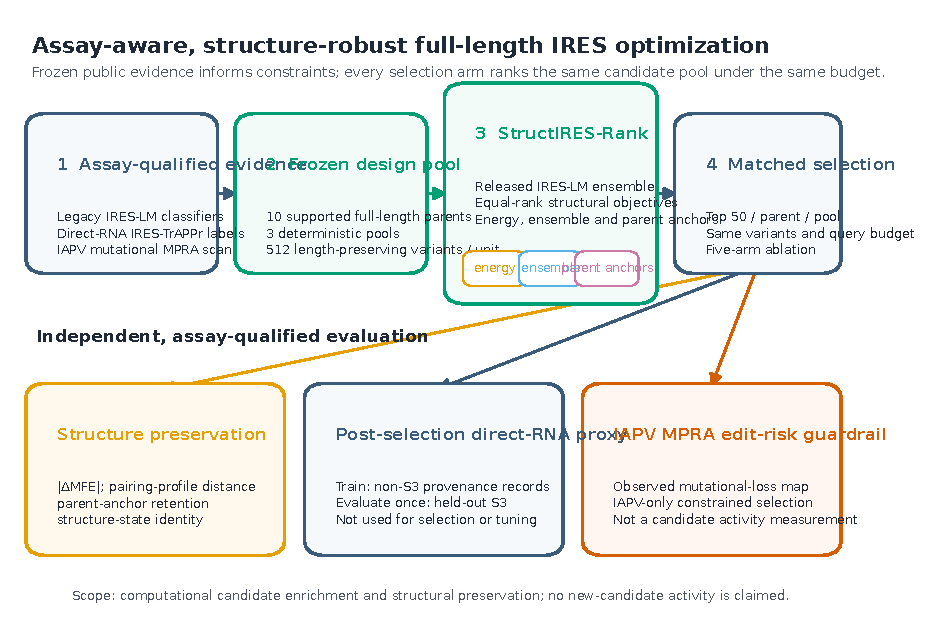
\includegraphics[width=0.98\textwidth]{figures/fig1_overview.pdf}
  \caption{Assay-labelled project route. The legacy identification benchmark is reproduced but is
  not treated as equivalent to direct-RNA activity. Full-length design is evaluated with independent
  function, structural-ensemble, cargo-context, applicability, and diversity criteria.}
  \label{fig:overview}
\end{figure*}

\begin{table}[t]
\centering
\caption{IRES-AI identification dataset recovered from the official split file.}
\label{tab:data}
\begin{tabular}{lrr}
\toprule
Source & Negative & Positive \\
\midrule
2016 synthetic library & 37,293 & 7,341 \\
IRESbase & 0 & 276 \\
IRESite combined & 120 & 249 \\
Rfam & 0 & 1,306 \\
IRESPred negatives & 189 & 0 \\
\midrule
Total & 37,602 & 9,172 \\
\bottomrule
\end{tabular}
\end{table}


\subsection{Identification benchmark}
On reconstructed nested folds, composition features already achieved AUC $0.710\pm0.009$ and AUPR
$0.405\pm0.015$, while hashed 3--6-mer features achieved AUC $0.723\pm0.011$ and AUPR
$0.452\pm0.016$. These are shortcut-control pilots rather than claims against published models.
Published reference values and project runs remain visibly separated in
Table~\ref{tab:prediction} and Figure~\ref{fig:prediction-pilot}.

\begin{figure*}[t]
  \centering
  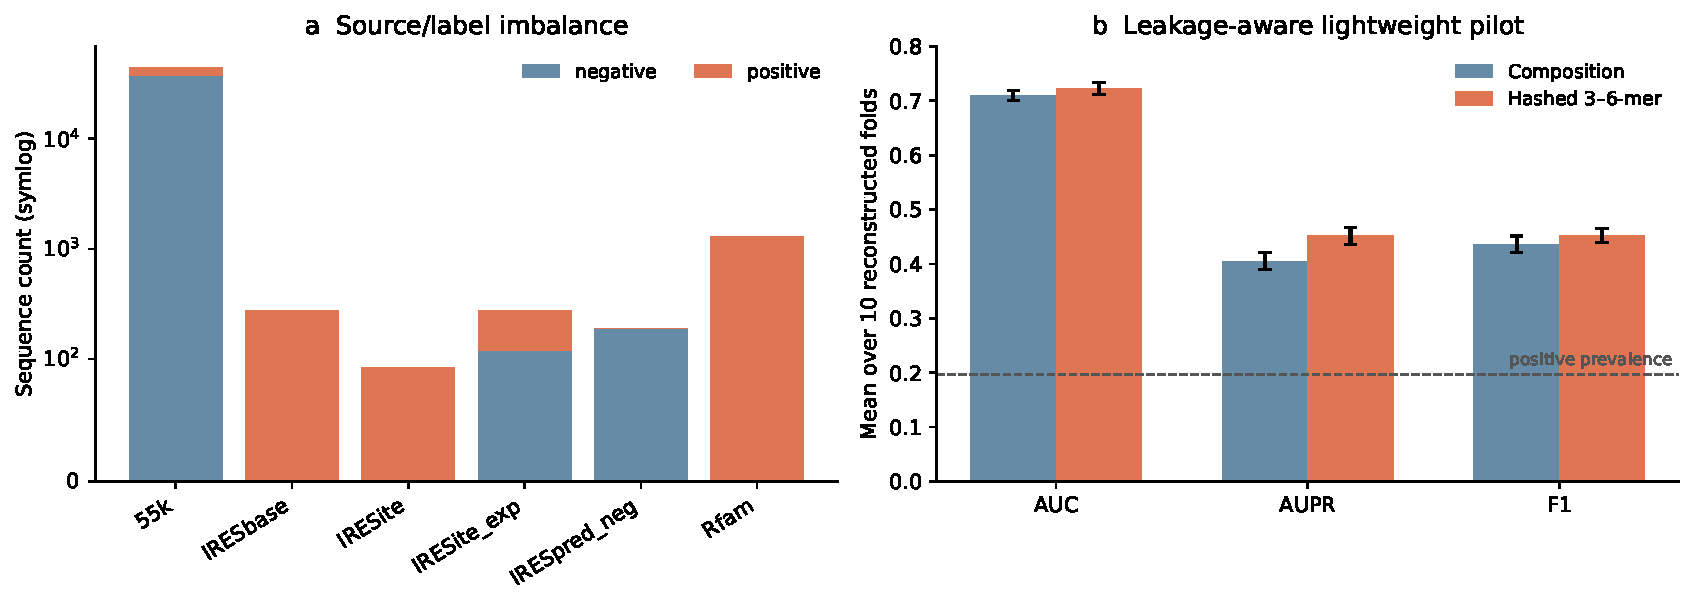
\includegraphics[width=0.98\textwidth]{figures/fig2_prediction_pilot.pdf}
  \caption{Dataset shortcut audit and leakage-aware lightweight pilot. Error bars show standard
  deviation over ten reconstructed test folds; the next fold is used only for threshold selection.
  Similarity-cluster results are intentionally pending.}
  \label{fig:prediction-pilot}
\end{figure*}

\begin{table*}[t]
\centering
\caption{IRES identification benchmark. Published values are references, not rerun results. Pilot
values are mean $\pm$ standard deviation over reconstructed nested folds and are not directly
comparable with the released repeated-holdout protocol.}
\label{tab:prediction}
\begin{tabular}{llccc}
\toprule
Status & Method & AUC & AUPR & F1 \\
\midrule
Published & RNA-FM & 0.779 & 0.615 & 0.506 \\
Published & UTR-LM & 0.765 & 0.581 & 0.493 \\
Published & RNA-BERT & 0.740 & 0.530 & 0.460 \\
Published & ERNIE-RNA & 0.670 & 0.350 & 0.330 \\
Published & Evo-2 & 0.610 & 0.310 & 0.330 \\
Published & IRES-LM & 0.770 & 0.600 & 0.500 \\
Published & DeepCIP & 0.730 & 0.500 & 0.270 \\
Published & IRESpy & 0.670 & 0.370 & 0.110 \\
Published & IRESfinder & 0.610 & 0.270 & 0.350 \\
\midrule
Project pilot, reconstructed & Composition logistic & .710$\pm$.009 & .405$\pm$.015 & .436$\pm$.016 \\
Project pilot, reconstructed & Hashed k-mer linear & .723$\pm$.011 & .452$\pm$.016 & .452$\pm$.013 \\
Project, cluster split & Local RNA-AR frozen probe & -- & -- & -- \\
Project, cluster split & Structure-aware model & -- & -- & -- \\
\bottomrule
\end{tabular}
\end{table*}


\subsection{Cross-assay transfer}
\textbf{Pending locked assay-shift run.} This section will report transfer and calibration rather
than selecting a favorable cross-assay subset.

\subsection{Constrained full-length optimization}
\textbf{Pending baseline gate.} The primary claim requires paired robust-full versus score-only
effects under identical candidate and oracle-query budgets.

\begin{table*}[t]
\centering
\caption{Matched ablation of \textsc{StructIRES-Rank} using the released IRES-LM ensemble
(mean of all ten RNA-FM and ten UTR-LM released classifiers). Values are mean $\pm$ sample SD
across 30 parent-by-run units (10 full-length IRES seeds $\times$ 3 frozen mutation pools); every
arm retains the top 50 of the same 512 candidates per unit. ``Anchor retention'' is the weighted
retention of parent-derived high-confidence ensemble base pairs ($P\geq0.5$), not an experimentally
mapped structural motif. The direct-RNA proxy is post-selection, S3-held-out and computational only.}
\label{tab:design}
\resizebox{\textwidth}{!}{%
\begin{tabular}{lcccccc}
\toprule
Selection method & $|\Delta$MFE| & Pairing $L_1$ & State identity & Anchor retention & Direct-RNA proxy & Role \\
\midrule
IRES-LM score-only & $4.021\pm1.254$ & $0.164\pm0.027$ & $0.798\pm0.048$ & $0.646\pm0.075$ & $0.419$ & Sequence baseline \\
+ energy rank & $0.647\pm0.196$ & $0.118\pm0.024$ & $0.857\pm0.042$ & $0.766\pm0.062$ & $0.427$ & Energy ablation \\
+ ensemble rank & $2.089\pm0.666$ & $0.055\pm0.014$ & $0.932\pm0.054$ & $0.915\pm0.026$ & $0.431$ & Ensemble ablation \\
+ anchor rank & $2.093\pm0.580$ & $0.062\pm0.015$ & $0.924\pm0.063$ & $0.920\pm0.028$ & $0.431$ & Anchor ablation \\
\textsc{StructIRES-Rank} & $0.666\pm0.226$ & $0.037\pm0.010$ & $0.954\pm0.049$ & $0.955\pm0.015$ & $0.435$ & Combined constraints \\
\bottomrule
\end{tabular}
}
\end{table*}


\subsection{Legacy 174-nt de novo benchmark}
IRES-DM released outputs are an external reference. A strict superiority claim requires retraining
under the shared data and budget protocol.
